% Options for packages loaded elsewhere
\PassOptionsToPackage{unicode}{hyperref}
\PassOptionsToPackage{hyphens}{url}
%
\documentclass[
]{article}
\usepackage{lmodern}
\usepackage{amssymb,amsmath}
\usepackage{ifxetex,ifluatex}
\ifnum 0\ifxetex 1\fi\ifluatex 1\fi=0 % if pdftex
  \usepackage[T1]{fontenc}
  \usepackage[utf8]{inputenc}
  \usepackage{textcomp} % provide euro and other symbols
\else % if luatex or xetex
  \usepackage{unicode-math}
  \defaultfontfeatures{Scale=MatchLowercase}
  \defaultfontfeatures[\rmfamily]{Ligatures=TeX,Scale=1}
\fi
% Use upquote if available, for straight quotes in verbatim environments
\IfFileExists{upquote.sty}{\usepackage{upquote}}{}
\IfFileExists{microtype.sty}{% use microtype if available
  \usepackage[]{microtype}
  \UseMicrotypeSet[protrusion]{basicmath} % disable protrusion for tt fonts
}{}
\makeatletter
\@ifundefined{KOMAClassName}{% if non-KOMA class
  \IfFileExists{parskip.sty}{%
    \usepackage{parskip}
  }{% else
    \setlength{\parindent}{0pt}
    \setlength{\parskip}{6pt plus 2pt minus 1pt}}
}{% if KOMA class
  \KOMAoptions{parskip=half}}
\makeatother
\usepackage{xcolor}
\IfFileExists{xurl.sty}{\usepackage{xurl}}{} % add URL line breaks if available
\IfFileExists{bookmark.sty}{\usepackage{bookmark}}{\usepackage{hyperref}}
\hypersetup{
  hidelinks,
  pdfcreator={LaTeX via pandoc}}
\urlstyle{same} % disable monospaced font for URLs
\usepackage[margin=1in]{geometry}
\usepackage{graphicx,grffile}
\makeatletter
\def\maxwidth{\ifdim\Gin@nat@width>\linewidth\linewidth\else\Gin@nat@width\fi}
\def\maxheight{\ifdim\Gin@nat@height>\textheight\textheight\else\Gin@nat@height\fi}
\makeatother
% Scale images if necessary, so that they will not overflow the page
% margins by default, and it is still possible to overwrite the defaults
% using explicit options in \includegraphics[width, height, ...]{}
\setkeys{Gin}{width=\maxwidth,height=\maxheight,keepaspectratio}
% Set default figure placement to htbp
\makeatletter
\def\fps@figure{htbp}
\makeatother
\setlength{\emergencystretch}{3em} % prevent overfull lines
\providecommand{\tightlist}{%
  \setlength{\itemsep}{0pt}\setlength{\parskip}{0pt}}
\setcounter{secnumdepth}{-\maxdimen} % remove section numbering

\author{}
\date{\vspace{-2.5em}}

\begin{document}

\startappendices

\hypertarget{chap:appendix_a}{%
\section{Backpropagation with Binary
Cross-Entropy}\label{chap:appendix_a}}

Let's consider a simple binary classification task. It is common to use
a network with a single logistic output with the binary cross-entropy
loss function and for the sake of simplicity, let's assume that there is
only one hidden layer. \[
\begin{aligned}
BCE=-\sum_{i=1}^{n o u t}\left(y_i \log \left(\hat{y}_i \right)+\left(1-y_i\right) \log \left(1-\hat{y}_i\right)\right)
\end{aligned}
\]

Where \(y\) is the ground truth and \(\hat{y}\) is the output of the
network. After having the loss function, let's continue with the forward
pass.

\[
\begin{aligned} 
a_{k} &= h_{k-1} w_{k} + b_k \\
h_k &= f(a_{k})
\end{aligned}
\]

Where, \(w_k\) is the weight, \(b_{k}\) is the bias term, \(h_k\) is the
output of the layer (which means that \(h_0 = X\) and \(h_2 = \hat{y}\))
and f is the non linear function. Please note that for last layer
logistic function is used whereas for hidden layer reLU is used as non
linear functions.\\
We can compute the derivative of the weights by using the chain rule.

\[
\begin{aligned} 
\frac{\partial BCE}{\partial w_{2}}=\frac{\partial BCE}{\partial \hat{y}} \frac{\partial \hat{y}}{\partial a_{2}} \frac{\partial a_{2}}{\partial w_{2}}
\end{aligned}
\]

Computing each factor in the term, we have: \[
\begin{aligned}
\frac{\partial BCE}{\partial \hat{y}} &=\frac{-y}{\hat{y}}+\frac{1-y}{1-\hat{y}} \\
&=\frac{\hat{y}-y}{\hat{y}\left(1-\hat{y}\right)} \\
\frac{\partial \hat{y}}{\partial a_{2}} &=\hat{y}\left(1-\hat{y}\right) \\
\frac{\partial a_{2}}{\partial w_{2}} &=h_{1}^T
\end{aligned}
\] Which gives us: \[
\frac{\partial BCE}{\partial w_{2}}=h_{1}^T\left(\hat{y}-y\right)
\] Derivative of the \(w_1\) concerning loss function can be calculated
as the following:

\[
\begin{aligned} 
\frac{\partial BCE}{\partial w_{1}}=\frac{\partial BCE}{\partial h_1} \frac{\partial h_1}{\partial a_{1}} \frac{\partial a_{1}}{\partial w_{1}}
\end{aligned}
\] Compute each factor in the term again, we have:

\[
\begin{aligned}
\frac{\partial BCE}{\partial h_1} &= \frac{\partial BCE}{\partial \hat{y}} \frac{\partial \hat{y}}{\partial a_{2}} \frac{\partial a_{2}}{\partial h_{1}}  \\
&= \left(\hat{y}-y\right) w_{2}^T \\
\frac{\partial h_1}{\partial a_{1}} &=f'(a_1) \\
\frac{\partial a_{1}}{\partial h_{1}} &=X^T
\end{aligned}
\] Which gives us: \[
\begin{aligned}
\frac{\partial BCE}{\partial w_{1}}= \left(X\right)^T\left(\hat{y}-y\right)\left(w_{2}^T\right) \odot f'(a_1)
\end{aligned}
\] Where \(\odot\) is element-wise multiplication, similarly, bias terms
can be calculated by following:

\[
\begin{aligned} 
\frac{\partial BCE}{\partial b_{2}}&=\frac{\partial BCE}{\partial \hat{y}} \frac{\partial \hat{y}}{\partial a_{2}} \frac{\partial a_{2}}{\partial b_{2}} \\
&= \left(\hat{y}-y\right)
\end{aligned}
\]

\[
\begin{aligned} 
\frac{\partial BCE}{\partial b_{1}}&=\frac{\partial BCE}{\partial h_1} \frac{\partial h_1}{\partial a_{1}} \frac{\partial a_{1}}{\partial b_{1}} \\
&= \left(\hat{y}-y\right)\left(w_{2}^T\right) \odot f'(a_1)
\end{aligned}
\] After having all these results, we can update the parameters (weights
and biases) using gradient descent and its variants.

\hypertarget{hidden-representation-of-digits-in-parity-problem}{%
\section{Hidden Representation of Digits in Parity
Problem}\label{hidden-representation-of-digits-in-parity-problem}}

On of the interesting question is: Does the network learn the digits
individually when we train the network and make the necessary processes
(summation, division) or does it memorize the way data is fed? This
question can be answered by observing the hidden representation. If the
network learns the digits well, we need to observe a well separation as
in MNIST task. For this purpose hidden representation of the networks
trained with BP and DFA are plotted in two dimensional space by using
t-SNE \cite{vanDerMaaten2008} implementation of sklearn
\cite{scikit-learn}.\\
Hidden representation of single image in \(k=3\) case is obtained as the
following way; we know that after we flatten the images, particular
parts of each images are multiplied corresponding parts of the weight
matrix. By getting these parts and performing multiplication for each
digit will gives us the hidden representation of the individual digit
that is trained in \(k=3\) case. Process is visualized in
\ref{fig:HiddenRepProcess}

\begin{figure}

{\centering 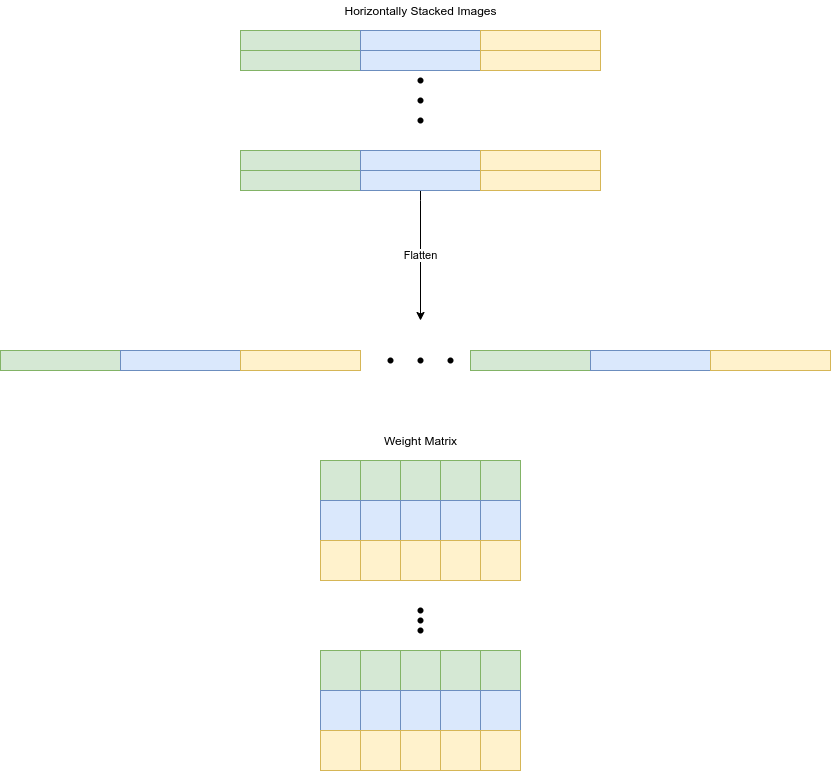
\includegraphics[width=1\linewidth]{../figures/hidden_rep_process} 

}

\caption{Process of Hidden Representation}\label{fig:HiddenRepProcess}
\end{figure}

\hypertarget{reproducibility}{%
\section{Reproducibility}\label{reproducibility}}

TODO: Write down the library versions, refer to the github repository
for the experiments, give information about the hardware. Explain the
stochastic behaviour of data.

\end{document}
